\documentclass[a4paper]{article}
\usepackage[utf8]{inputenc}
\usepackage[russian,english]{babel}
\usepackage[T2A]{fontenc}
\usepackage[left=10mm, top=20mm, right=18mm, bottom=15mm, footskip=10mm]{geometry}
\usepackage{indentfirst}
\usepackage{amsmath,amssymb}
\usepackage[italicdiff]{physics}
\usepackage{graphicx}
\graphicspath{{images/}}
\DeclareGraphicsExtensions{.pdf,.png,.jpg}
\usepackage{wrapfig}
\usepackage{pgfplots}

\usepackage{caption}
\captionsetup[figure]{name=Рисунок}
\captionsetup[table]{name=Таблица}


\title{\underline{Лабораторная работы 2.2.6}}
\author{Старостин Александр, Б01-401}
\date {11 февраля, 2025 год}


\begin{document}

\maketitle
\newpage

\textbf{Определение энергии активации по температурной зависимости вязкости жидкости}

\section{Аннотация}
    \par \textbf{Цель работы:} 1) измерение скорости падения шариков при разной температуре жидкости; 2) вычисление вязкости жидкости по закону Стокса и расчёт энергии активации.\\

    \par \textbf{В работе используются:} стеклянный цилиндр с исследуемой жидкостью (глицерин); термостат; секундомер; горизонтальный компаратор; микроскоп; мелкие шарики (диаметром около 1 мм).


\section{Теоретическая часть}
    \subsection{Энергия активации}
    Для того чтобы перейти в новое состояние, молекула жидкости должна преодолеть участки с большой потенциальной энергией, превышающей среднюю тепловую энергию молекул. Для этого тепловая энергия молекул должна — вследствие флуктуации — увеличиться на некоторую величину $W$ , называемую энергией активации. Температурная зависимость вязкости жидкости при достаточно грубых предположениях можно описать формулой
    \begin{equation} \label{activation_energy:1}
        \eta = A e^{W/kT}
    \end{equation}

    Из формулы (\ref{activation_energy:1}) следует, что существует линейная зависимость между величинами $ln\eta$ и $1/T$, и энергию активации можно найти по формуле

    \begin{equation} \label{activation_energy:2}
        W = k \frac{d(ln\eta)}{d(1/T)}
    \end{equation}

    \subsection{Измерение вязкости}
    По формуле Стокса, если шарик радиусом $r$ и со скоростью $v$ движется в среде с вязкостью $\eta$, и при этом не наблюдается турбулентных явлении, тормозящую силу можно найти по формуле (\ref{stokes})

    \begin{equation}\label{stokes}
        F = 6\pi\eta \frac{d}{2}v
    \end{equation}


    Для измерения вязкости жидкости рассмотрим свободное падение шарика в жидкости. При медленных скоростях на шарик действуют силы Архимеда и Стокса, выражения для которых мы знаем. Отсюда находим выражения для установившейся скорости шарика и вязкости жидкости

    \begin{align}
        v_{уст}&=\frac{2}{9}g\frac{d^2}{4}\frac{\rho - \rho_ж}{\eta}\label{v_ust}\\
        \eta&=\frac{2}{9}g\frac{d^2}{4}\frac{\rho - \rho_ж}{v_{уст}}\label{eta}
    \end{align}

    Как видим, измерив установившуюся скорость шарика и параметры системы можно получить вязкость по формуле (\ref{eta}).

    \subsection{Экспериментальная установка}
    Для измерений используется стеклянный цилиндрический сосуд B, наполненный исследуемой жидкостью (глицерин). Диаметр сосуда $\approx 3$ см, длина $\approx 25$ см. На стенках сосуда нанесены две метки на некотором расстоянии друг от друга. Верхняя метка должна располагаться ниже уровня жидкости с таким расчетом, чтобы скорость шарика к моменту прохождения этой метки успевала установиться. Измеряя расстояние между метками, b время падения определяют установившуюся скорость шарика $v_{уст}$. Сам сосуд B помещен в рубашку D, омываемую водой из термостата. При работающем термостате температура воды в рубашке D, а потому и температура жидкости 12 равна температуре воды в термостате.
    Схема прибора (в разрезе) показана на рис.~\ref{ustanovka}.
    \begin{figure}[ht]
        \center{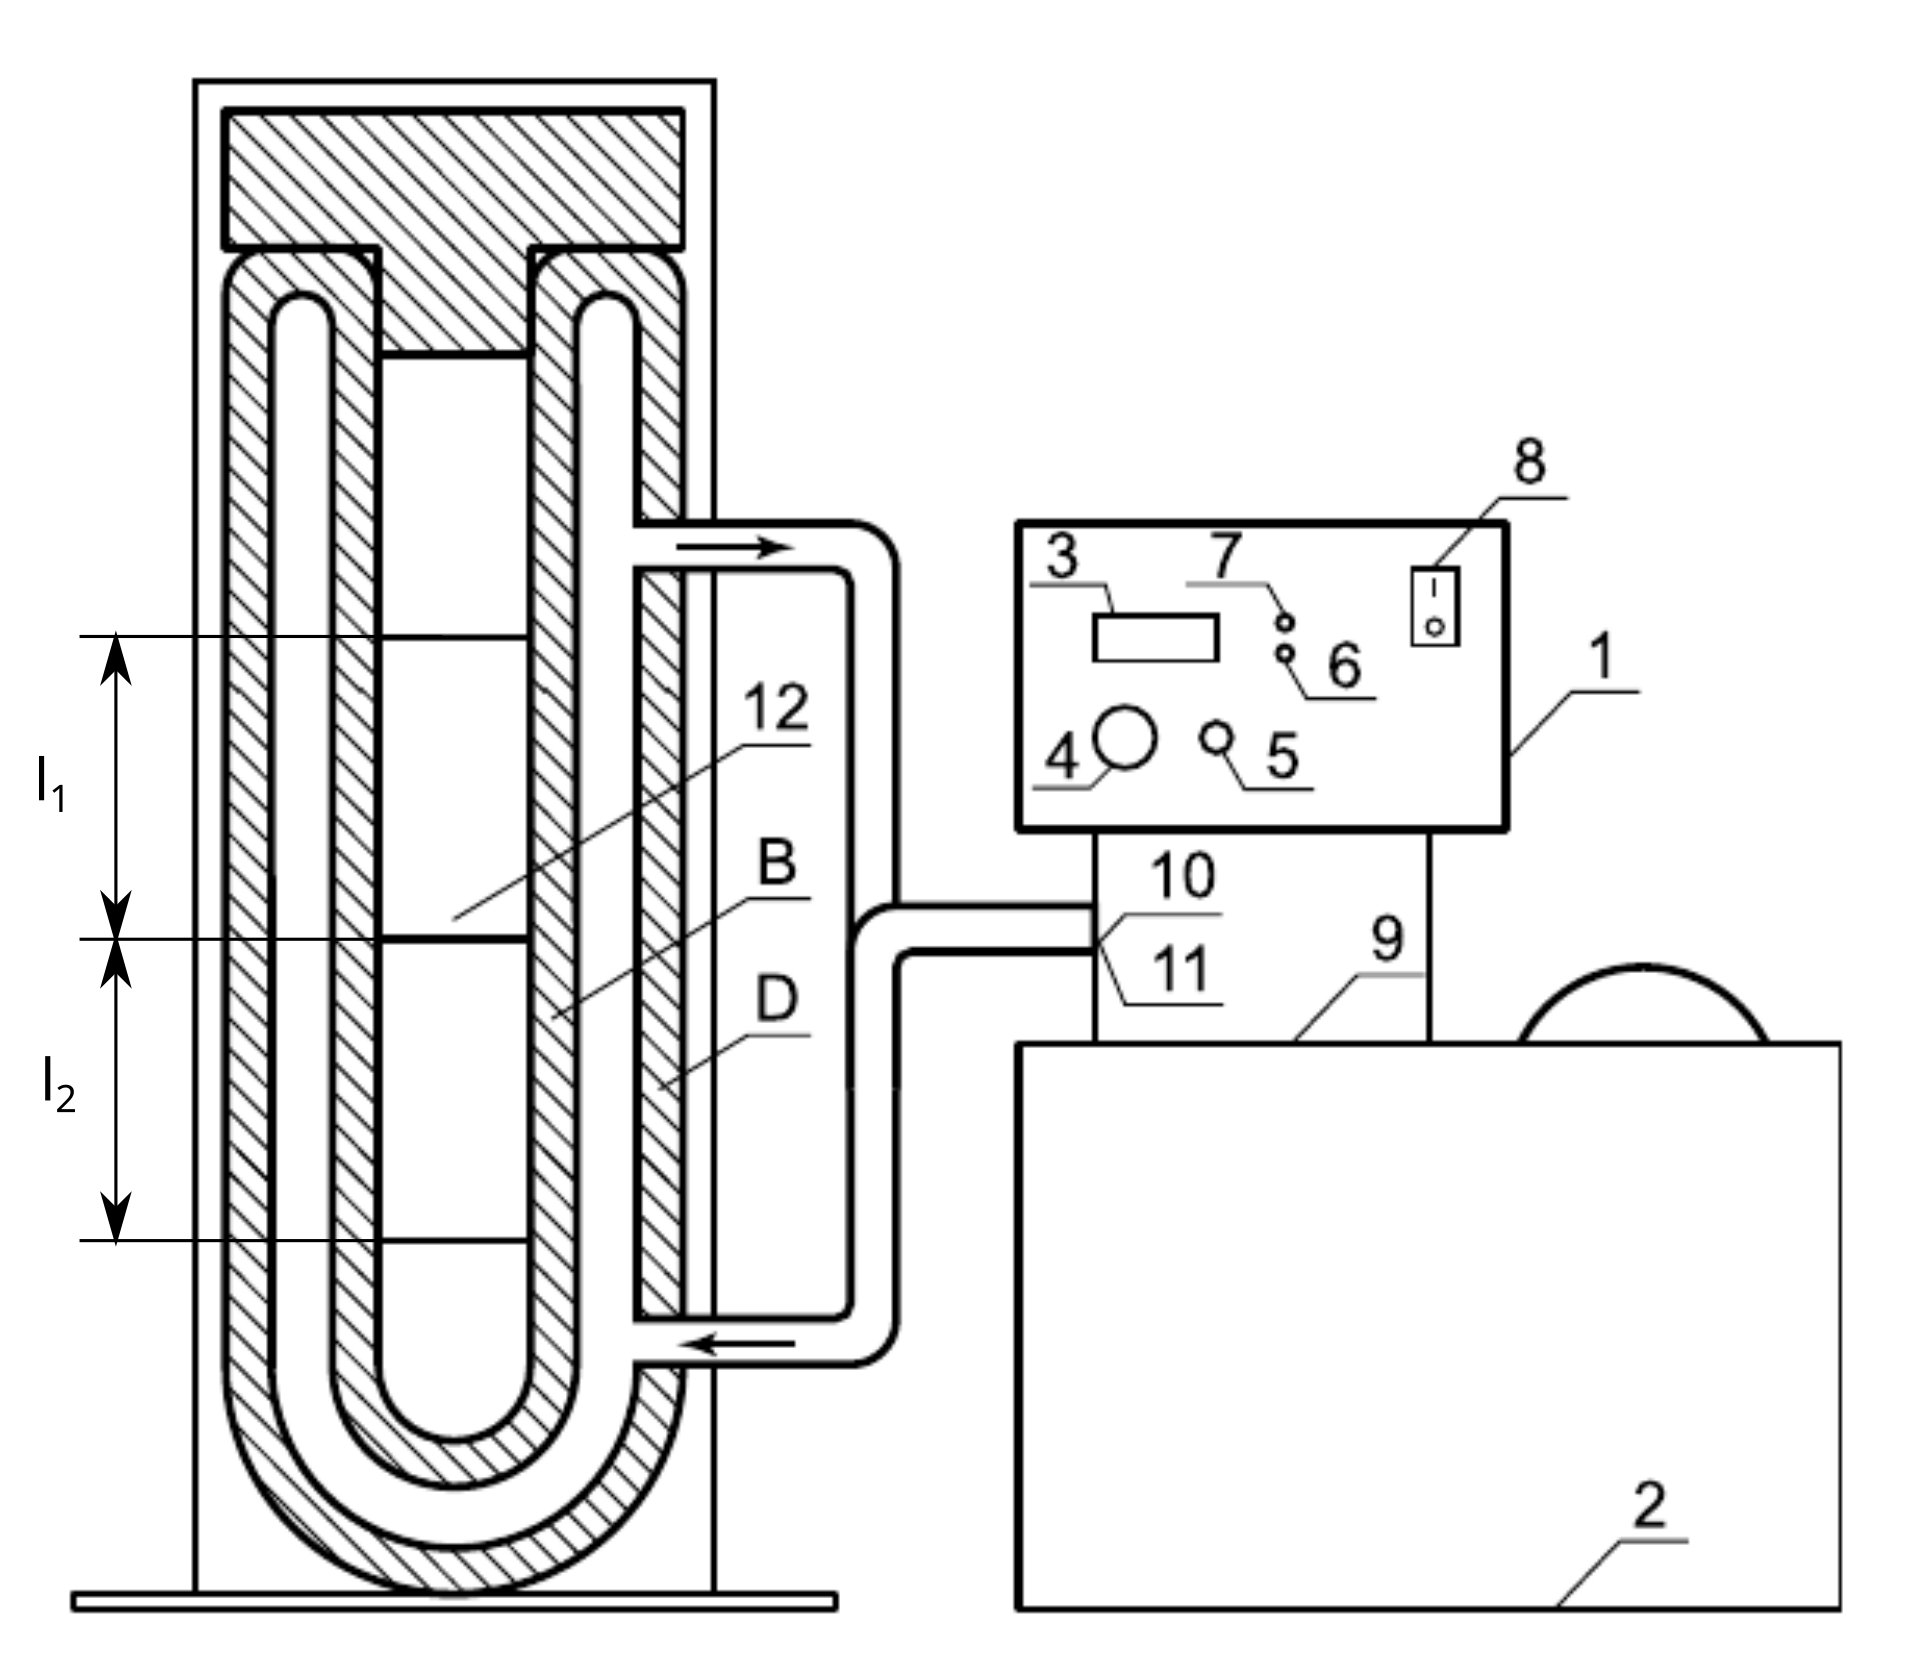
\includegraphics[scale=0.5]{ustanovka}}
        \caption{Установка для определения коэффициента вязкости жидкости.}
        \label{ustanovka}
    \end{figure}

\newpage

    \subsection{Другие формулы}

    Время рeлаксации:
    \begin{equation}
        \tau = \frac{2d^2\rho}{9*4\eta}
    \end{equation}

    Путь рeлаксации:
    \begin{equation}
        S = v\tau
    \end{equation}

\section{Ход работы}

\subsection{Измерение диаметра шариков}

Отберём 10 стальных и 10 стеклянных шариков различного размера и с помощью микроскопа измерим их средние размеры. Данные измерений приведены в таблице~\ref{diameters}. Приборная погрешность измерений $\sigma_\text{d приб} = 0.02 \text{мм}$.
    \begin{table}[!ht]
        \centering
        \subtable{
            \begin{tabular}{|c|c|c|}
            \hline
                № & Материал & Диаметр, мм \\ \hline
                1  & Стекло & 1,94 \\ \hline
                2  & Стекло & 2,02 \\ \hline
                3  & Стекло & 1,78 \\ \hline
                4  & Стекло & 1,98 \\ \hline
                5  & Стекло & 1,96 \\ \hline
                6  & Стекло & 1,92 \\ \hline
                7  & Стекло & 1,96 \\ \hline
                8  & Стекло & 1,96 \\ \hline
                9  & Стекло & 1,98 \\ \hline
                10 & Стекло & 1,94 \\ \hline
            \end{tabular}
        }
        \subtable{
            \begin{tabular}{|c|c|c|}
            \hline
                № & Материал & Диаметр, мм \\ \hline
                1  & Сталь & 0,76 \\ \hline
                2  & Сталь & 0,72 \\ \hline
                3  & Сталь & 0,76 \\ \hline
                4  & Сталь & 0,80 \\ \hline
                5  & Сталь & 0,68 \\ \hline
                6  & Сталь & 0,72 \\ \hline
                7  & Сталь & 0,72 \\ \hline
                8  & Сталь & 0,76 \\ \hline
                9  & Сталь & 0,72 \\ \hline
                10 & Сталь & 0,76 \\ \hline
            \end{tabular}
        }
        \caption{Измеренные диаметры шариков}
        \label{diameters}
    \end{table}

    Плотности шариков равны: $\rho_\text{стекло}=(2.5 \pm 0.1) \text{ г/см}^3$ и $\rho_\text{сталь}=(7.8 \pm 0.1) \text{ г/см}^3$\\

    Получаем, что: $\overline{d_\text{стекло}} = 1,94\text{ мм}$ и $\overline{d_\text{сталь}} = 0,76 \text{ мм}$\\

    Случайная погрешность: $\sigma_\text{сл} = \sqrt{\frac{\sum_i^n(d_i - \overline{d})^2}{n(n-1)}}$

    $\sigma_\text{сл стекло} = 0,02\text{ мм}$

    $\sigma_\text{сл сталь} =  0,01\text{ мм}$\\

    Полная погрешность: $\sigma_d = \sqrt{\sigma_\text{d случ}^2 + \sigma_\text{d приб}^2}$

    $\sigma_\text{стекло} = 0,03\text{ мм}$

    $\sigma_\text{сталь} =  0,02\text{ мм}$


    \subsection{Измерение установившихся скоростей падения шариков}

    Измеренные длины цилиндра установки (см. рис.~\ref{ustanovka}): $l_1 = l_2 = (10.0 \pm 0.1)\text{ см}$ \\

    Измерения произведём для 5 значений температуры от 25 до 50 $ ^\circ C $. При помощи секундомера измерим время прохождения шариком участков $l_1$ ($ \sigma_t = 0.3\text{ с}$). Вычисляем установившуюся скорость шариков в жидкости. По графику на рис.~\ref{density} определим плотность глицерина для каждой температуры. По формуле~(\ref{eta}) рассчитываем вязкость глицерина. Примем $g = (9.81 \pm 0.01)\text{ м/с}^2$. Результаты представлены в таблице (2).

    \begin{figure}[ht]
        \center{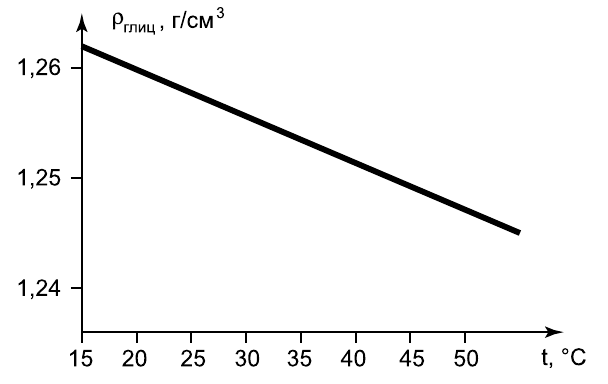
\includegraphics[scale=0.5]{density.png}}
        \caption{График плотности глицерина в зависимости от температуры.}
        \label{density}
    \end{figure}


    \begin{table}[h!]
    \centering
    \begin{tabular}{|c|c|c|c|c|c|c|c|c|c|}
    \hline
    №  & $\text{темп, }^\circ C$  & $T\text{, K}$ & $\rho_\text{гл} \text{, г/см}^{3}$ & $\text{материал}$ & $t\text{, с}$ & $\upsilon$ \text{, см/с} & $\tau$ $\text{, с}$ & $S\text{, см}$ & $\eta\text{, Па*с}$   \\ \hline

    1  & $20$ & $293$ & $1,260$ & сталь  & $53,7$ & 0,19 & 2,02  & 0,38 & 1,24 \\ \hline
    2  &      &       &         & сталь  & $43,1$ & 0,23 & 2,75  & 0,63 & 0,91 \\ \hline
    3  &      &       &         & стекло & $38,3$ & 0,26 & 5,33  & 1,39 & 0,98 \\ \hline
    4  &      &       &         & стекло & $34,7$ & 0,29 & 5,94  & 1,72 & 0,88 \\ \hline

    5  & $30$ & $303$ & $1,256$ & сталь  & $21,1$ & 0,47 & 5,33  & 2,51 & 0,47 \\ \hline
    6  &      &       &         & сталь  & $20,4$ & 0,49 & 5,56  & 2,73 & 0,45 \\ \hline
    7  &      &       &         & стекло & $21,8$ & 0,46 & 9,50  & 4,37 & 0,55 \\ \hline
    8  &      &       &         & стекло & $20,0$ & 0,50 & 10,25 & 5,12 & 0,51 \\ \hline

    9  & $40$ & $313$ & $1,253$ & сталь  & $13,2$ & 0,76 & 7,82  & 5,94 & 0,32 \\ \hline
    10  &      &       &         & сталь  & $14,4$ & 0,69 & 7,36  & 5,08 & 0,34 \\ \hline
    11  &      &       &         & стекло & $10,6$ & 0,94 & 19,36 & 18,20 & 0,27 \\ \hline
    12  &      &       &         & стекло &  $9,1$ & 1,10 & 22,73 & 25,00 & 0,23 \\ \hline

    13  & $45$ & $318$ & $1,249$ & сталь  & $10,1$ & 0,99 & 11,92 & 11,80 & 0,21 \\ \hline
    14  &      &       &         & сталь  &  $6,3$ & 1,59 & 19,25 & 30,62 & 0,13 \\ \hline
    15  &      &       &         & стекло &  $6,2$ & 1,61 & 32,67 & 52,60 & 0,16 \\ \hline
    16  &      &       &         & стекло &  $5,8$ & 1,72 & 34,85 & 59,94 & 0,15 \\ \hline

    17  & $50$ & $323$ & $1,247$ & сталь  &  $5,0$ & 2,00 & 25,03 & 50,06 & 0,10 \\ \hline
    18  &      &       &         & сталь  &  $4,0$ & 2,50 & 31,29 & 78,22 & 0,08 \\ \hline
    19  &      &       &         & стекло &  $4,1$ & 2,44 & 47,52 & 115,95 & 0,11 \\ \hline
    20  &      &       &         & стекло &  $4,2$ & 2,38 & 47,52 & 113,10 & 0,11 \\ \hline

    \end{tabular}
    \caption{Результаты измерений установившихся скоростей шариков и соответствующих плотностей глицерина}
    \end{table}

    Погрешности:

    $\sigma_T = 0.3 \text{ K}$

    $\sigma_{\rho} = 0.001\text{ г/см}^3$

    $\sigma_v = v\sqrt{\left( \frac{\sigma_l}{l}\right)^2 + \left(\frac{\sigma_{t}}{t} \right)^2}$

    $\sigma_{\eta} = \eta \sqrt{\left( \frac{\sigma_g}{g}\right)^2 + \left( 2\frac{\sigma_d}{d}\right)^2 + \left( \frac{\sigma_{v}}{v}\right)^2 + \frac{\sigma_{\rho}^2 + \sigma_{\rho_{глиц}}^2}{(\rho - \rho_{глиц})^2}}$


    Средняя относительная погрешность измерений вязкости $\varepsilon_{\eta} = 9.5\% $

    \subsection{Оценка времени и пути релаксации. Анализ применимости формулы Стокса}

    Все результаты представлены в таблице (2).

    \begin{align}
        \tau &= \frac{2}{9} \frac{d^2}{4} \frac{\rho}{\eta}, & \varepsilon_{\tau} &= \sqrt{\left( 2\frac{\sigma_d}{d} \right)^2  + \left( \frac{\sigma_{\rho}}{\rho} \right)^2 + \left( \frac{\sigma_{\eta}}{\eta} \right)^2}\label{relax_time}\\
        S &= v_{уст} \tau, & \varepsilon_S &= \sqrt{\left( \frac{\sigma_{v_{уст}}}{v_{уст}} \right)^2  + \left( \frac{\sigma_{\tau}}{\tau} \right)^2}\label{S}
    \end{align}

    Тогда:

    \begin{align*}
        \langle \varepsilon_{\tau} \rangle &= 10.8\%, & \langle \varepsilon_S \rangle &= 6.2\%
    \end{align*}

    Как видим, во всех экспериментах путь релаксации пренебрежимо мал. Следовательно формула Стокса применима.

    \subsection{График зависимости $ln \eta$ от $1/T$}

    \begin{figure}[ht]
        \center{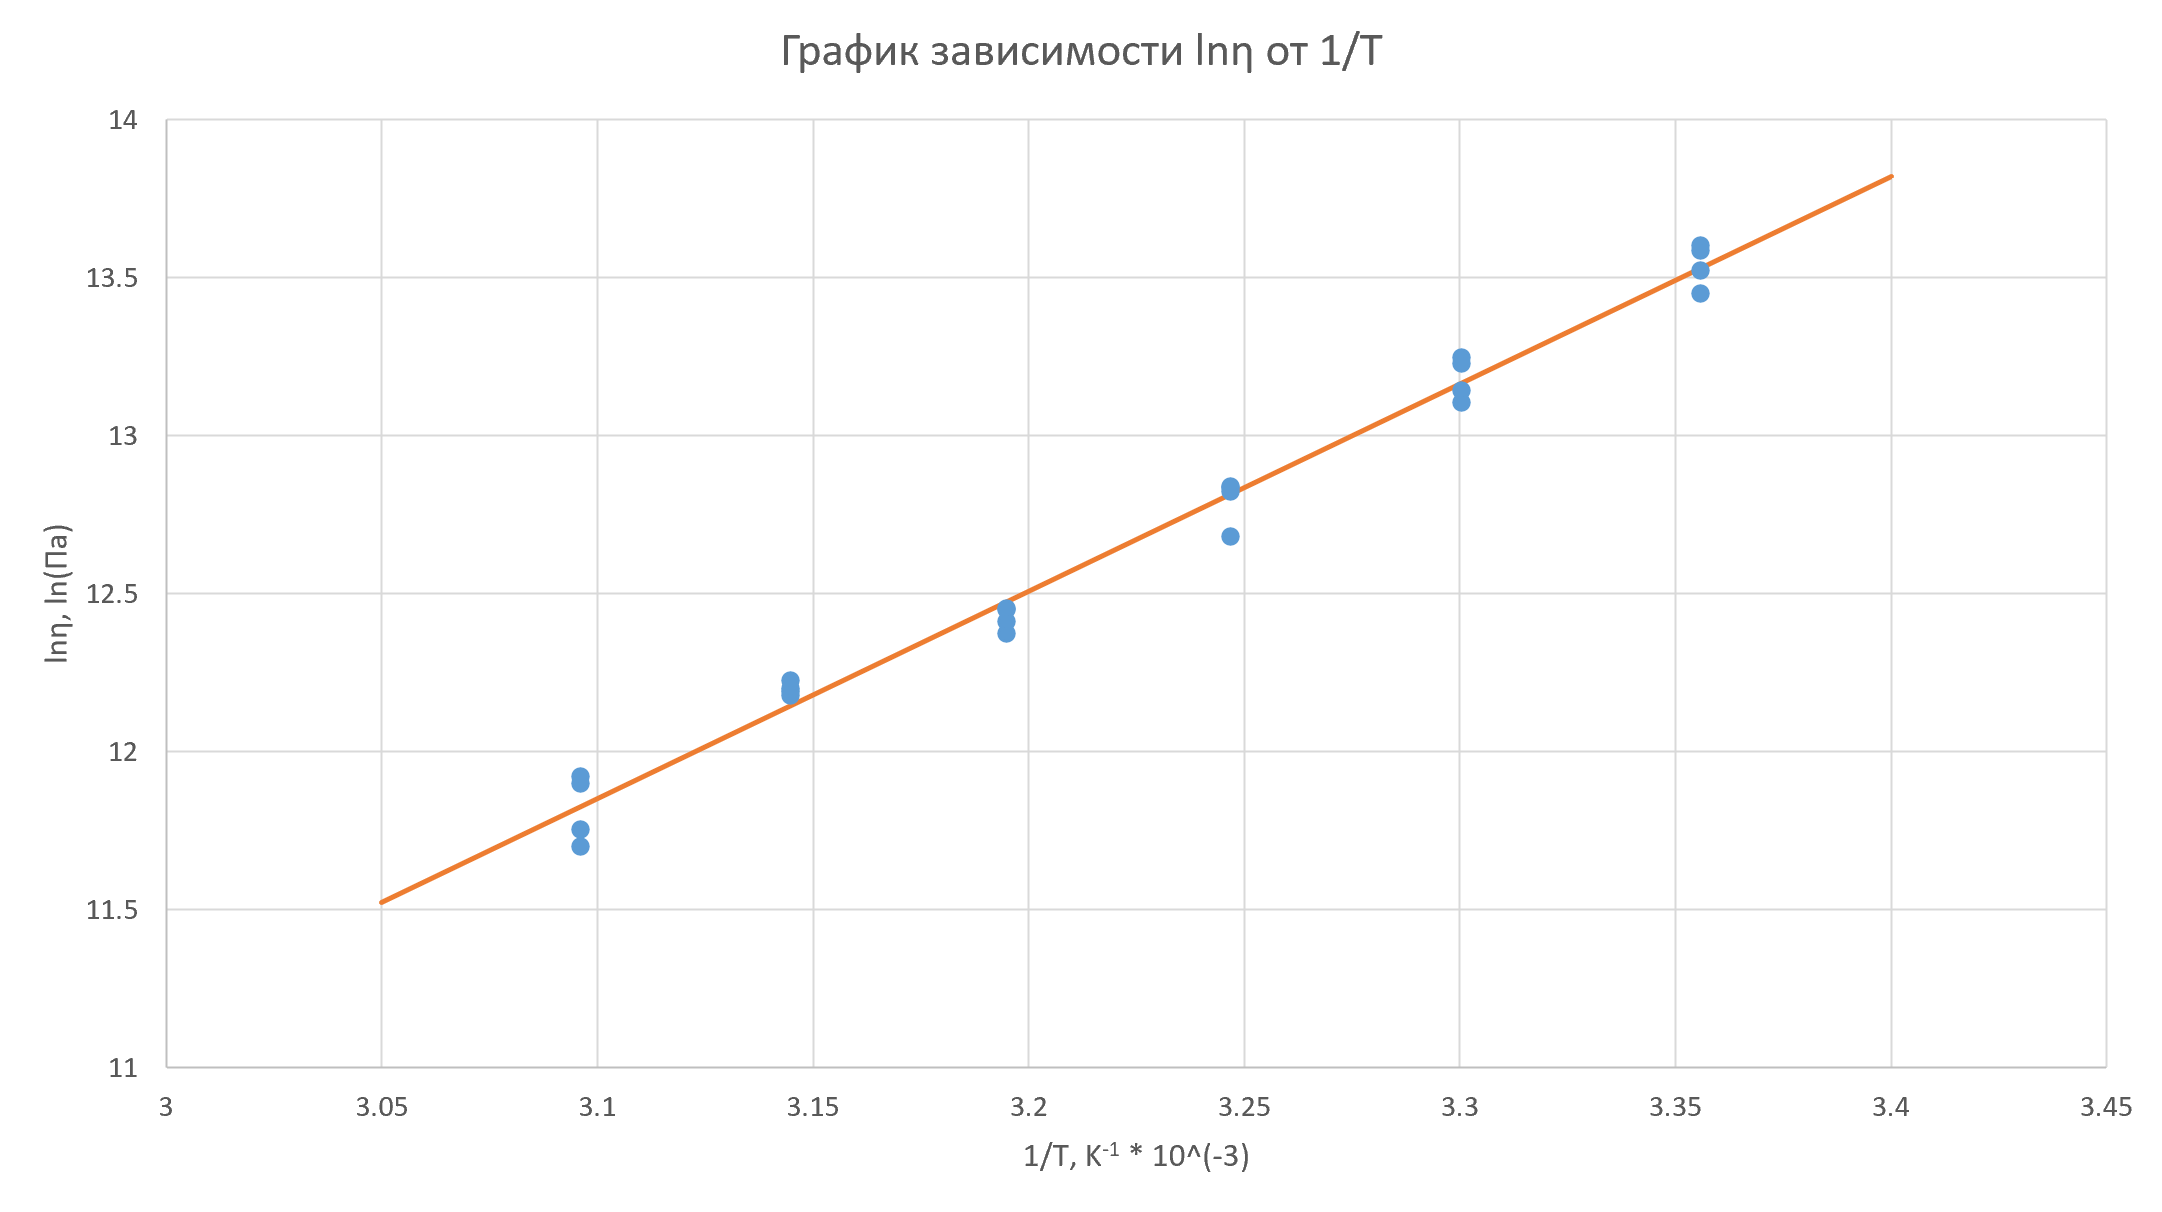
\includegraphics[scale=0.8]{graph.png}}
        \caption{График зависимости $ln \eta$ от $1/T$.}
        \label{graph}
    \end{figure}

    По методу наименьших квадратов вычислим угол наклона прямой.

    \begin{align*}
        k_{накл} = \frac{\langle xy \rangle - \langle x \rangle \langle y \rangle}{\langle x^2 \rangle - \langle x \rangle^2} = (6570 \pm 160) \text{ K}
    \end{align*}

    Прямая, полученная по МНК не проходит через 0. Это объясняется тем, что в формуле (\ref{activation_energy:1}) есть константа $A$. Коэффициент $b$ прямой соответственно равен $lnA$.

    \subsection{Вычисление энергии активации}

    При помощи формулы (\ref{activation_energy:2}) рассчитаем энергию активации:

    \begin{align*}
        W = k * k_\text{накл} = 1.38 * 10^{-23} \text{ Дж/К} * 6570 \text{ К} = 9.07 * 10^{-20} \text{ Дж}
    \end{align*}

    \subsection{Оценка погрешностей}

    Случайная погрешность энергии активации:

    \begin{align*}
        \sigma_{k_{накл}} &= \frac{1}{\sqrt{20}} \sqrt{\frac{\langle y^2 \rangle - {\langle y \rangle}^2}{\langle x^2 \rangle - {\langle x \rangle}^2} - k_{накл}^2} = 160~K\\
        \sigma_W^{случ} &= W \frac{\sigma_{k_{накл}}}{k} = 9.07 * 10^{-20} \text{ Дж} * 2.4\% = 0.218 * 10^{-20} \text{ Дж}
    \end{align*}

    Приборная погрешность энергии активации:

    \begin{align*}
        \sigma_W^{приб} &= W \sqrt{\left( \frac{\sigma_T}{T} \right)^2 + \left( \frac{\sigma_{\eta}}{\eta ln \frac{\eta}{A}} \right)^2} = 0.010 * 10^{-20}\text{ Дж}
    \end{align*}

    Полная погрешность энергии активации:

    \begin{align*}
        \sigma_W &= \sqrt{{\sigma_W^{приб}}^2 + {\sigma_W^{случ}}^2} = 0.037* 10^{-20}\text{ Дж}\\
        \varepsilon_W &= 2.5\%
    \end{align*}

    \section{Вывод}

    \begin{align*}
        W = (9.07 \pm 0.04) * 10^{-20} \text{ Дж}
    \end{align*}

    Измерили скорости падения шариков при разной температуре жидкости, вычислили вязкость жидкости по закону Стокса и рассчитали энергию активации.
\end{document}
